\chapter{Low temperature photoluminescence of $WS_2$}

\section{Introduction}

As the temperature of the semiconductor goes down the number of charge carriers decreases. Because of this in $WS_2$ the number of electrons is expected to be lower at low temperatures. Additionally as the temperature drops the peak broadening due to temperature effects i.e. Gaussian broadening decreases. At room temperature the thermal energy is equal to about 25 meV which limits the smallest possible width of the peak and therefore the resolution. Both of those effects should result in the peak at low temperatures to be overall weaker and more narrow than that at the room temperature. Additionally the lower electron density should result in lower population of trions. Due to lower temperature the electron and hole mobility should also decrease and cause the excitons to be more often trapped at defects sites also known as bound excitons.

\section{Experimental}

In order to perform the low temperature measurement the sample was placed in an environmental stage, Linkam THMS350V. The stage allows the sample to be cooled down to the temperatures of liquid nitrogen ($LN_2$) and at pressures of down to $10^{-3}$ mbar. The stage was then placed in a Renishaw Raman spectroscope chamber and the spectra were collected using 532nm green laser.

\section{Results}

The PL measurements were taken from the $WS_2$ monolayer on $Si/SiO_2$ sample at different conditions. As seen in Figure \ref{fig:LowTPLComparison} the PL from has been measured in the same spot at lower pressure ($2 \times 10^{-2}$ mbar) and different temperatures, room temperature and liquid nitrogen ($LN_2$) temperature ($-196 \degree C$). The PL from that spot at room temperature is centred at 1.957 eV and has FWHM of 44.3 meV. After lowering the temperature to that of $LN_2$ i.e. $-196 \degree C$ the PL measurement was taken again and the intensity of the peak was found to be about 0.81 that of the RT. Additionally the position of the PL at lower temperature was found to be 1.969 eV and the FWHM was 37.9 eV.

\begin{figure}[!ht]
	\begin{center}
		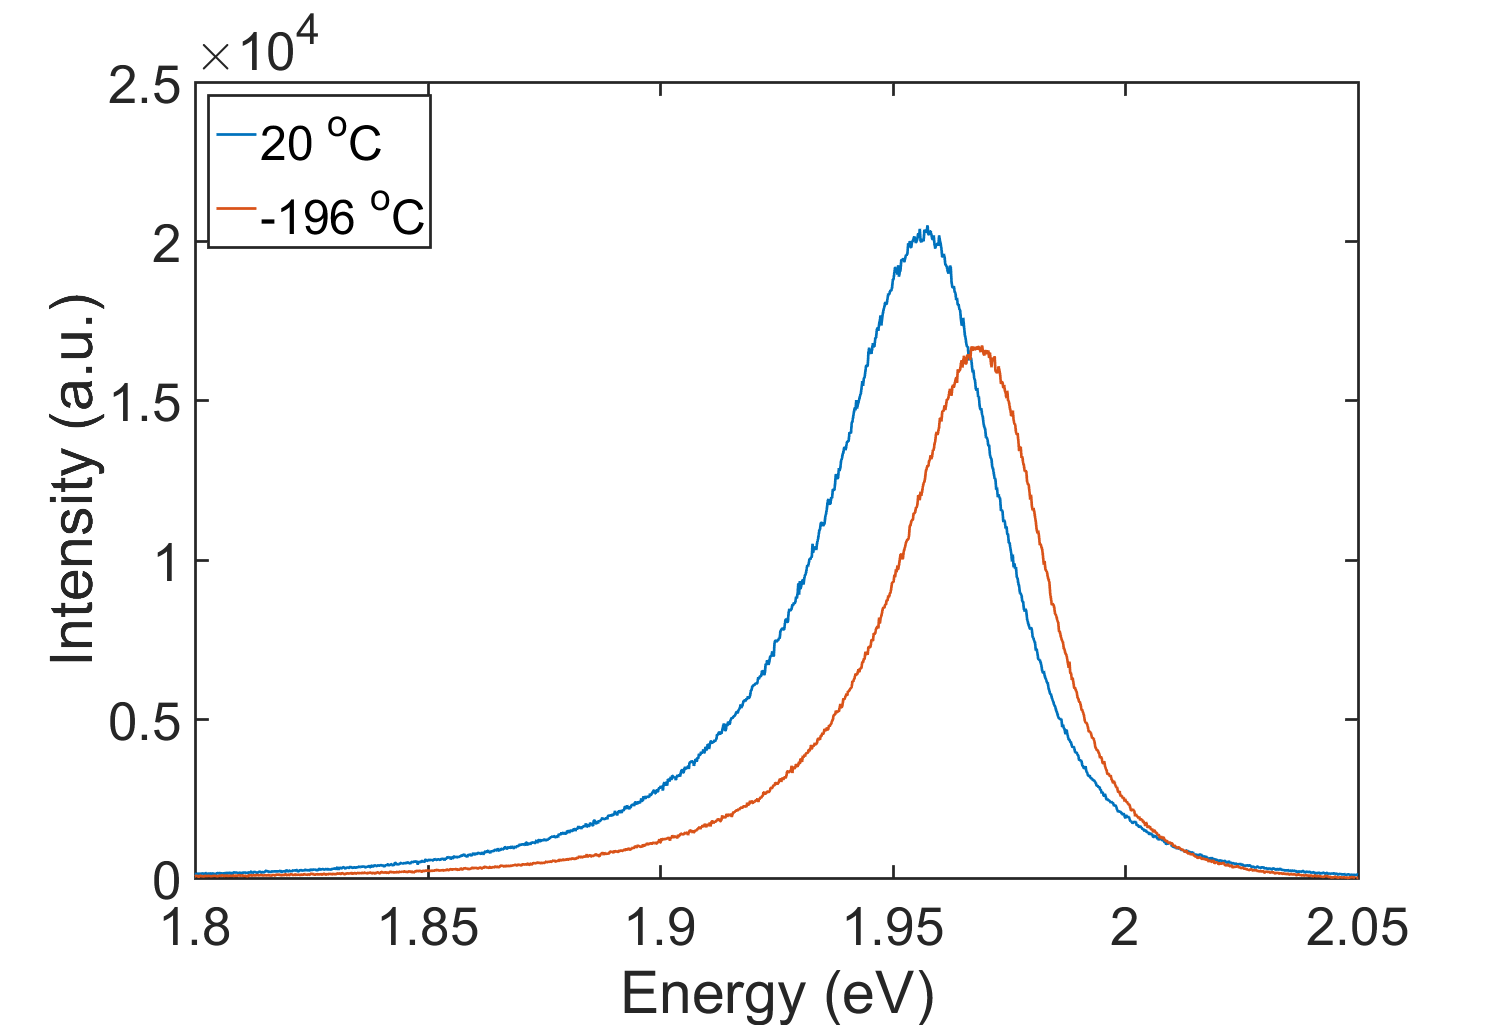
\includegraphics[scale=0.4]{LowT/LowTPLComparison.png}
		\caption{PL spectra of samples at room temperature and $LN_2$ temperature at $2 \times 10^{-2}$ mbar}
		\label{fig:LowTPLComparison}
	\end{center}
\end{figure}

The PL spectra were then fitted with 2 peaks to resolve the trions and excitons. The results can be seen in Figure \ref{fig:LowTPLDeconvolution}. Similarly the PL spectrum from room temperature has been fitted with two peaks. The intensity ratio between the exciton and trion in the low temperature sample is about 4, while at the room temperature it is 3. The FWHM of the exciton peak also lowers from 36 meV to about 32 meV.

This indicates that indeed as the temperature is lowered the FWHM of the PL peak and especially the exciton component also lowers. However the difference between the FWHM at room temperature and low temperature is not as big as expected if temperature was the main contributor to the peak broadening. For room temperature a thermal energy contribution should be about 25 meV while at $LN_2$ temperature (77 K) the contribution should be about half of that, i.e. 12 meV. The peak was fitted mostly with Gaussian lineshape (about 70\%) and therefore the temperature should be a significant contributor to the peak width. It is possible that the laser heats up the sample during measurement since the thermal contact between the substrate and the cooled stage is weak. Additionally the glass window separating the stage and the room environment as well as the substrate itself can be covered in water droplets which could introduce refraction and therefore peak broadening.  

\begin{figure}[!ht]
	\begin{center}
		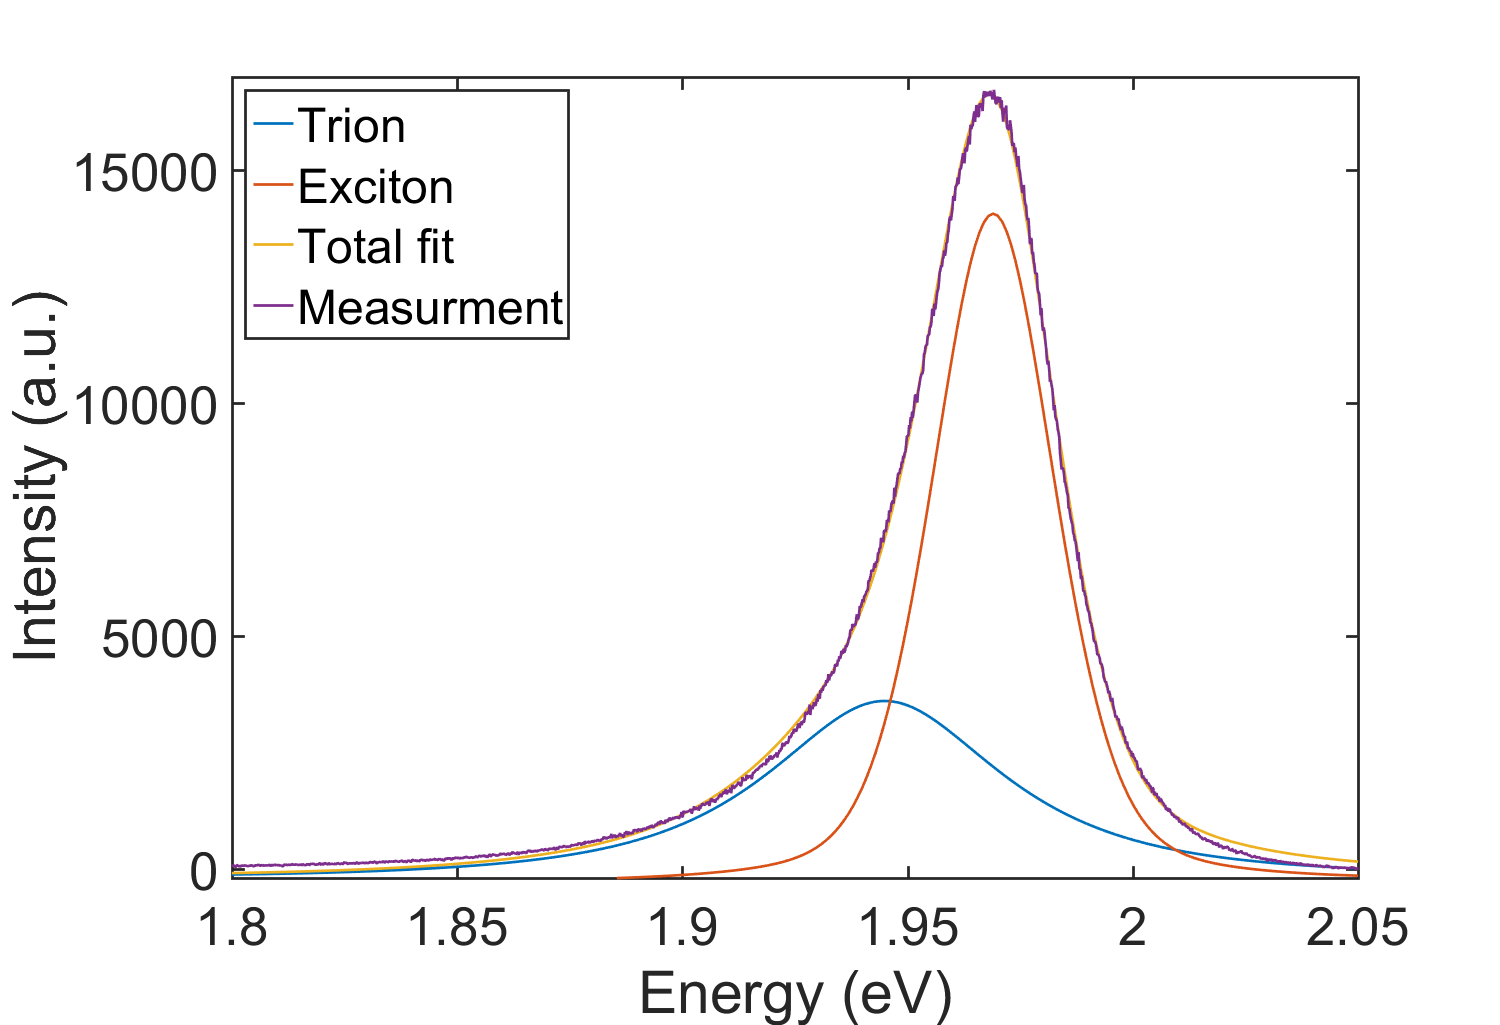
\includegraphics[scale=0.4]{LowT/LowTPLDeconvolution.png}
		\caption{PL spectra at low temperature with trions and excitons components resolved}
		\label{fig:LowTPLDeconvolution}
	\end{center}
\end{figure}

Due to the low FWHM of the PL peaks a strong trion component can be observed as seen in Figure \ref{fig:LowTPLStrongTrion}. While the lower temperature of the substrate can explain the small FWHM, the trion component is much stronger than in standard measurement environment. This could be caused by the low pressure which results in less oxygen and water molecules adsorbed at the defect sites. At standard conditions (1 atm) these species adsorb at the defect sites and attract electrons which as a result lowers the overall n-doping level of the material. 

\begin{figure}[!ht]
	\begin{center}
		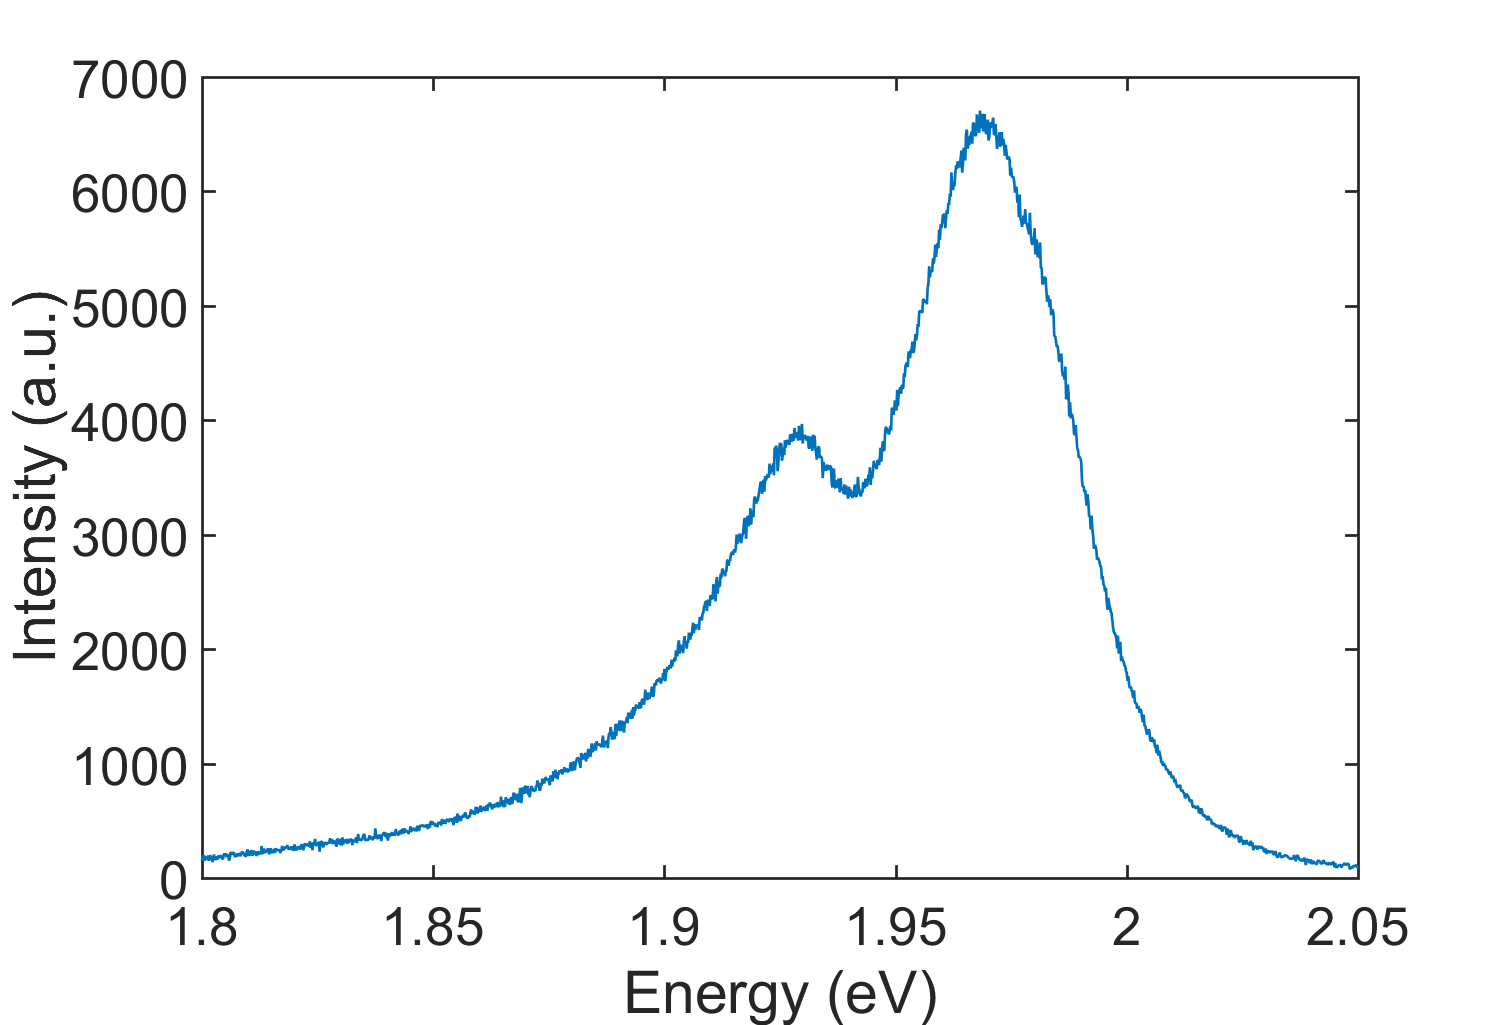
\includegraphics[scale=0.4]{LowT/LowTPLStrongTrion.png}
		\caption{Low temperature PL spectrum with easily resolved strong trion component}
		\label{fig:LowTPLStrongTrion}
	\end{center}
\end{figure}

In order to check the influence of the pressure on the PL and potential effect of the adsorbed oxygen, nitrogen and water molecules measurement at different pressures was conducted. As seen in Figure \ref{fig:LowTPLPressureDifference} as the pressure is lowered by several orders of magnitude the PL peak is shifted to the red. The FWHM of the PL peak at the ambient pressure is about 41 meV while at lower pressure ($1.5 \times 10^{-2}$ mbar) it is about 44 meV. The exciton to trion intensity ratio changes from 3.387 to 3.25 from the ambient pressure to low pressure. It therefore indicates that as the pressure is lowered the trion component becomes more prominent and the peak overall shifts to lower energies. 

\begin{figure}[H]
	\begin{center}
		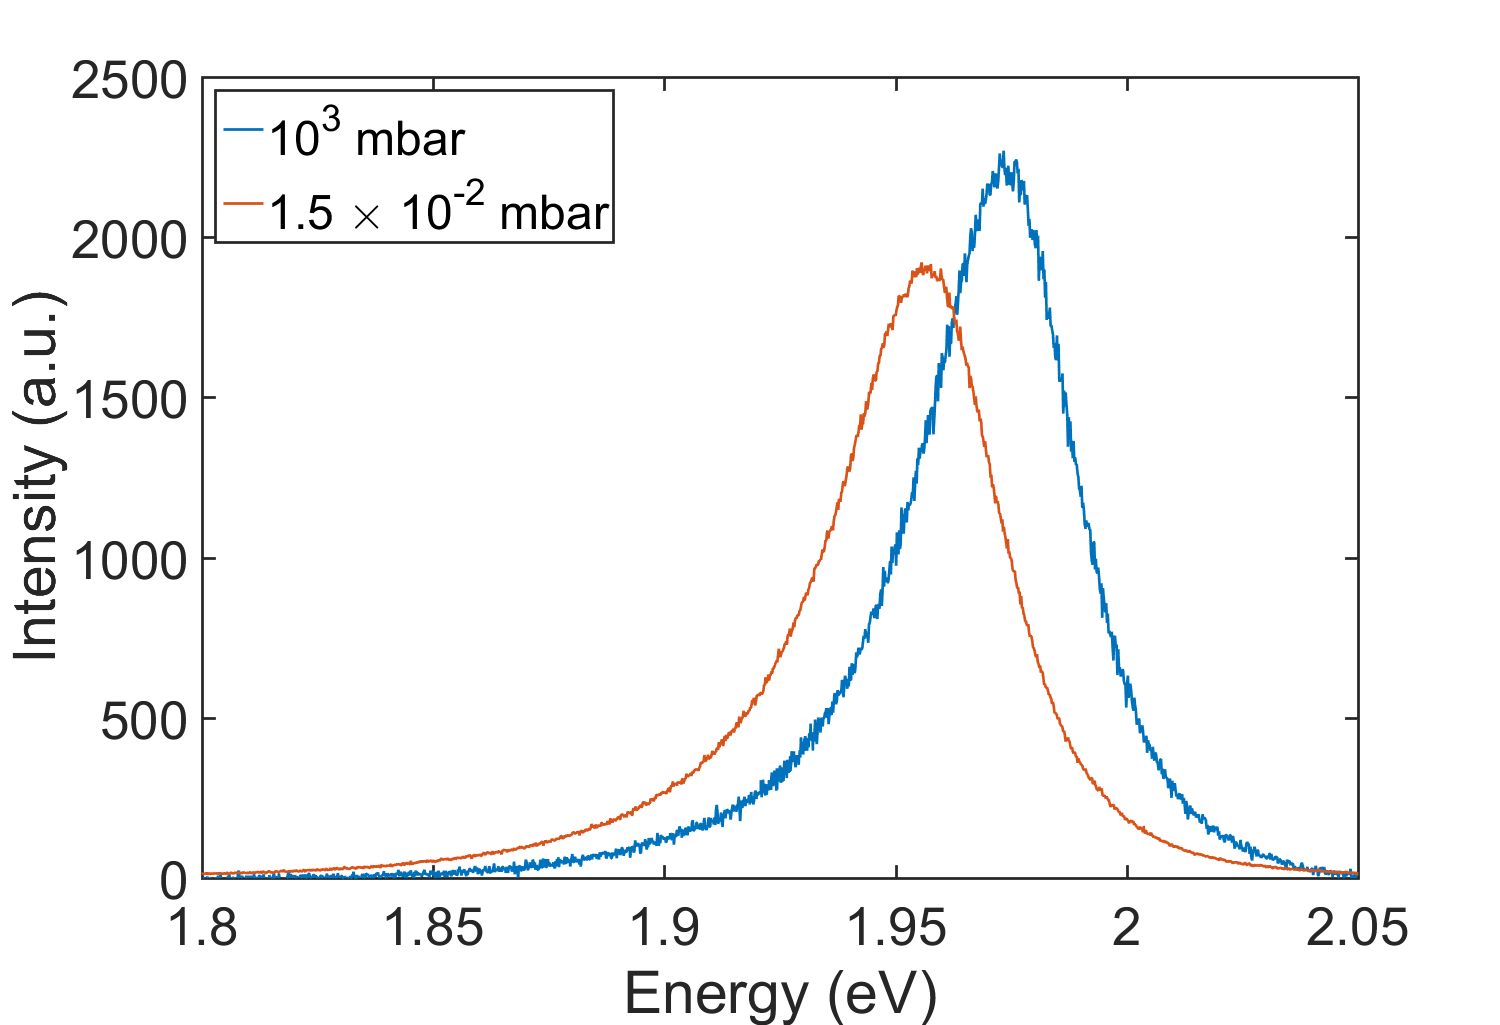
\includegraphics[scale=0.4]{LowT/LowTPLPressureDifference.png}
		\caption{PL measurements at different atmospheric pressures}
		\label{fig:LowTPLPressureDifference}
	\end{center}
\end{figure}

\section{Conclusions}

In this chapter we have reported PL investigation of CVD grown 2H $WS_2$ flakes at -196 {\degree}C temperature. By lowering the temperature we would expect to observe a sharpening of the excitonic transition and thus the possibility distinguish between excitons and trions quasiparticles as contributing to the PL.